\documentclass[12pt,a4paper]{article}

% -------------------
% MARK: Packages
% -------------------

% import geometry package to update the document margins
\usepackage[margin=1in]{geometry}
% set the font to helvectica
\usepackage[scaled]{helvet}
\renewcommand\familydefault{\sfdefault}
% for type-setting
\usepackage{amsmath, amssymb, amsfonts, verbatim, pifont}
% for slashed out text
\usepackage[normalem]{ulem}
% for units and scientific notation
\usepackage[table]{xcolor}
\usepackage{siunitx}
% for references and URLs
\usepackage{hyperref, url}
% Natbib setup for author-year style
\usepackage{natbib}
 \bibpunct[, ]{(}{)}{,}{a}{}{,}%
 \def\bibfont{\small}%
 \def\bibsep{\smallskipamount}%
 \def\bibhang{24pt}%
 \def\newblock{\ }%
 \def\BIBand{and}%
% for graphics and figures
\usepackage{graphicx, subfig, tikz}
% force figures to stay in their sections
\usepackage[section]{placeins}
% for tables
\usepackage{booktabs, longtable, tabularx}
\usepackage{multicol, multirow}
\usepackage{adjustbox}
\usepackage[flushleft]{threeparttable}
% a package for working with .csv data for tables
\usepackage{csvsimple}
% setup the algorithm package
% ruled: show bars around title and bar at bottom
% lined: show the line column on the left of the algorithm
% linesnumbered: print line numbers for each line
\usepackage[ruled,lined,linesnumbered]{algorithm2e}
\DontPrintSemicolon % don't print the semicolon that \; usually prints
% fix overfull hbox errors from oddities like using
% quotes (``foo'') and etc.
\usepackage{microtype}

% -------------------
% MARK: Debugging Packages
% -------------------

% import a debugging package to show the margin boxes
% \usepackage{showframe}

% -------------------
% MARK: Declarations
% -------------------

% setup captions for tables and figures
\captionsetup[table]{%
  labelfont={bf},
  name={Table},
  labelsep=colon,
  justification=raggedright,
  singlelinecheck=false}
\captionsetup[figure]{%
  labelfont={bf},
  name={Figure},
  labelsep=colon,
  justification=raggedright,
  singlelinecheck=false}
\captionsetup[algorithm2e]{%
  labelfont={bf},
  name={Figure},
  labelsep=colon,
  justification=raggedright,
  singlelinecheck=false}

% set the graphics path to the img directory
\graphicspath{{img/}}

% -----------------------------------------------------------------------------
% MARK: algorithm2e stuff
% -----------------------------------------------------------------------------

% params
% \SetKwInOut{Objects}{$\CKmatrix{O}$}
% \SetKwInOut{Weights}{$\CKvector{w}$}

% -------------------
% MARK: Headers
% -------------------

% headers and footers
\usepackage{fancyhdr}
\setlength{\headheight}{15pt}
\pagestyle{fancy}
\lhead{KautenjaDSP}
\rhead{\itshape RackNES v1.3.0}
\cfoot{\thepage}

% start the document
\begin{document}

% -------------------
% MARK: Title Page
% -------------------

% fancyhdr directive to remove headers from this title page
\thispagestyle{empty}
% center the title page contents
\vspace*{\fill}
\begin{center}

\includegraphics[width=0.8\textwidth]{RackNES-Logo}
\linebreak\linebreak\linebreak\linebreak
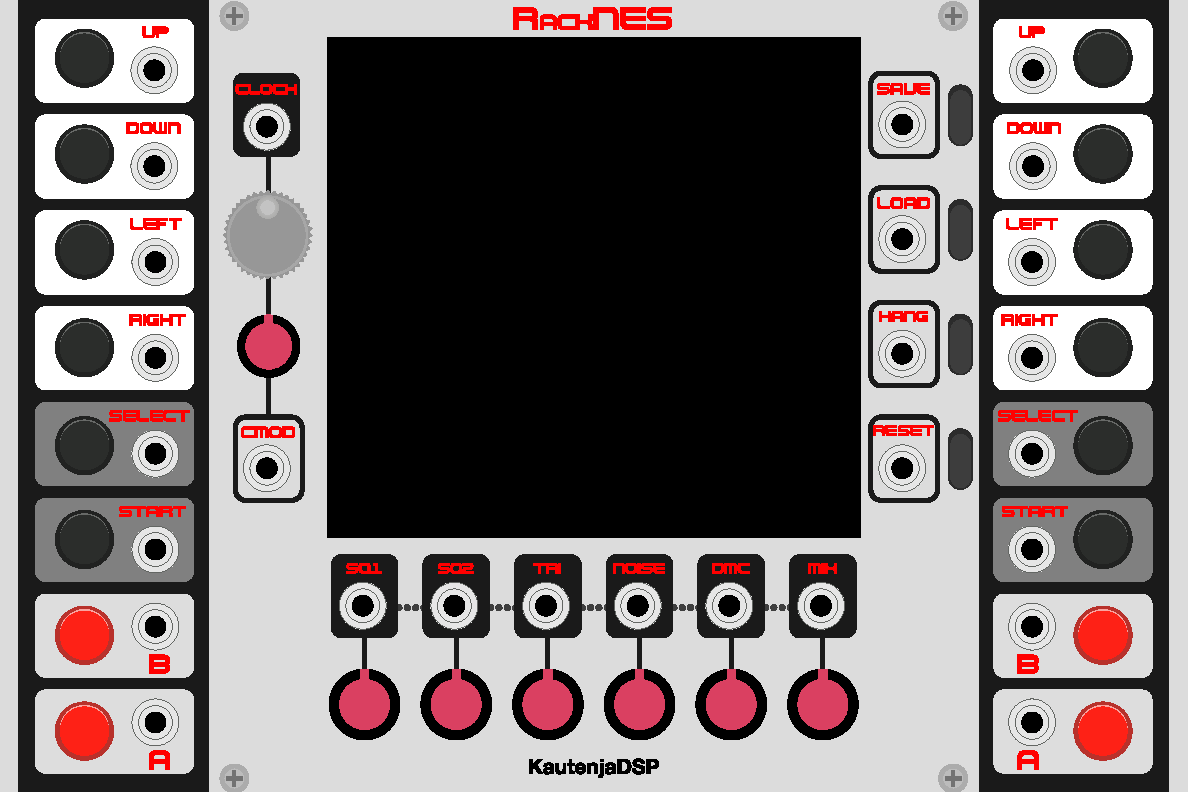
\includegraphics[width=0.8\textwidth]{RackNES-Module}
\linebreak\linebreak\linebreak\linebreak

\includegraphics[width=0.8\textwidth]{KautenjaDSP}
\end{center}
\vspace*{\fill}
\clearpage

% -------------------
% MARK: Overview
% -------------------

\section{Overview}

RackNES is a Nintendo Entertainment System (NES) emulator for VCV Rack with control voltage inputs and outputs. RackNES offers several key features, namely,

\begin{itemize}
  \item \textbf{Clock Source:} Use NES frame-rate (FPS) as a clock source for downstream modules;
  \item \textbf{Clock Rate Modulation:} Control the clock rate of the NES with direct knob and CV;
  \item \textbf{NES Audio Output:} Sample audio from the NES in real-time at any sampling rate;
  \item \textbf{Sampling/Ratcheting:} Save and restore the NES state for interesting musical effects;
  \item \textbf{Full CV Control:} CV inputs for Reset, Player 1, Player 2, and more; and
  \item \textbf{Channel Mixer:} Control the volume level of individual synthesizer channels.
\end{itemize}

% -------------------
% MARK: Loading ROMs
% -------------------

\section{Loading ROMs}

To load a game into RackNES:
\begin{enumerate}
  \item acquire a ROM dump of the desired game in the iNES format, the file-type will be \texttt{.NES} or \texttt{.nes};
  \item bring up the RackNES context menu by right-clicking the module and selecting ``\textbf{Load ROM}'';
  \item use the resulting file explorer to locate the ROM file from (1) and load it into RackNES;
  \item if the ROM file is invalid or cannot be loaded, RackNES will inform you using a pop-up dialog.
\end{enumerate}

% -------------------
% MARK: Mappers
% -------------------

\section{Mappers}

Unlike digital media, NES games were deployed using cartridges based on functioning circuits. These cartridges often had special logical mappings, or else employed additional resources (e.g., ROM, RAM, ASICs) to extend the capabilities of the NES. These mappers must be individually accounted for in the emulation of the NES in order to support the games that use them. Otherwise, the code for those games will not execute correctly, if at all. RackNES supports many of the common mappers, with plans to support more in the future. Table~\ref{tab:mappers} outlines which mappers are supported by the current stable release of RackNES.

\begin{table}[!htp]
\centering
\begin{tabular}{|l|l|}
 \hline
 ID & Name   \\
 \hline\hline
 0  & NROM   \\
 \hline
 1  & MMC1   \\
 \hline
 2  & UNROM  \\
 \hline
 3  & CNROM  \\
 \hline
\end{tabular}
\caption{NES mappers supported by the current release of RackNES.}
\label{tab:mappers}
\end{table}

% -------------------
% MARK: Panel Layout
% -------------------

\section{Panel Layout}

\begin{figure}[!htp]
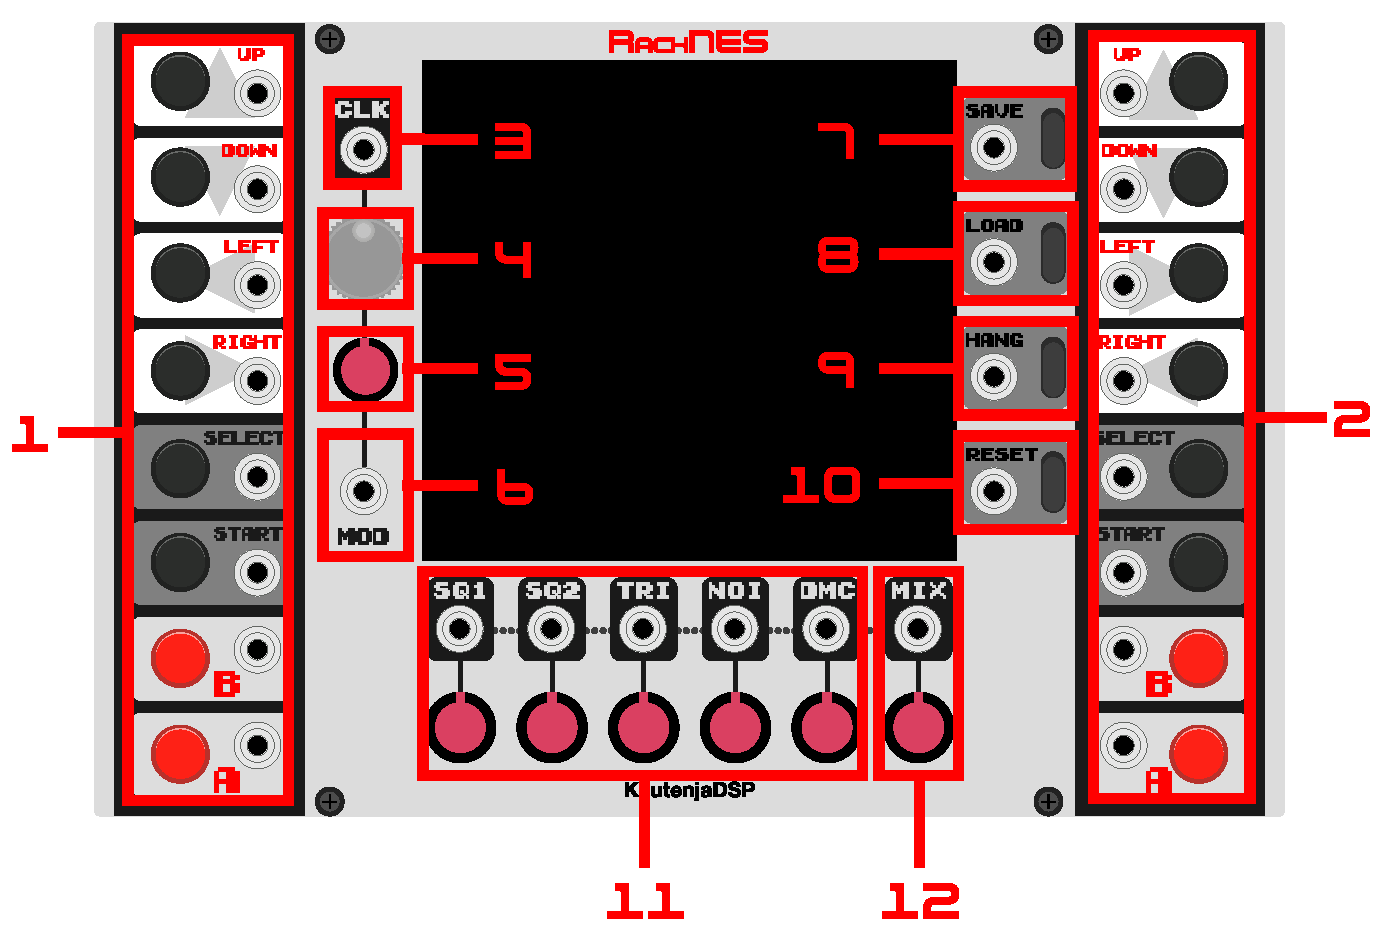
\includegraphics[width=\textwidth]{RackNES-Manual}
\end{figure}

\begin{enumerate}
  \item Player 1 controller input gates; high at $2V$
  \item Player 2 controller input gates; high at $2V$
  \item NES Clock output. A pulse wave with $50\%$ duty cycle; high at $10V$, low at $0V$. Rising edge follows the frame-rate of the NES where a frame occurs once every $29781$ CPU cycles, i.e., $f_{output} = \frac{f_{clock}}{29781}$
  \item NES Clock rate control. Controls the clock rate of the NES starting at a base rate of $f_{clock} = 1.7898MHz$.
  \item NES Clock rate CV attenuverter. Controls strength and polarity of clock rate CV input.
  \item NES Clock rate CV modulation. Modulates the clock rate parameter according to CV with half the range of the clock rate control knob.
  \item Save state trigger; high at $2V$. Saves the current state of emulation.
  \item Load state trigger; high at $2V$. Loads the existing save state back into the emulation.
  \item Hang emulation trigger; high at $2V$. Causes the emulation to hold state when the gate is high.
  \item Reset emulator trigger; high at $2V$. Equal to pressing "Reset" on the NES, resets the game.
  \item NES Channel Mixer. Outputs and level controls for each of the five synthesis channels on the NES; $10V_{pp}$. Channels are removed from the global mix when connected. Knobs controls the gain of the audio output signal from $0\%$ to $200\%$.
  \item NES Mix output; $10V_{pp}$. Sum of the five synthesis channels NES. Channels with connected outputs are removed from the mix. The knob controls the gain of the audio output signal from $0\%$ to $200\%$.
\end{enumerate}

% -------------------
% MARK: References
% -------------------

\clearpage
\renewcommand\refname{References \& Acknowledgments}
\nocite{*}
\bibliographystyle{apalike}
\bibliography{references}

\end{document}
